\documentclass[12pt]{article}

\usepackage{graphicx}
\usepackage{paralist}
\usepackage{amsfonts}
\usepackage{amsmath}
\usepackage{hhline}
\usepackage{booktabs}
\usepackage{multirow}
\usepackage{multicol}
\usepackage{url}

\oddsidemargin -10mm
\evensidemargin -10mm
\textwidth 160mm
\textheight 200mm
\renewcommand\baselinestretch{1.0}

\pagestyle {plain}
\pagenumbering{arabic}

\newcounter{stepnum}

%% Comments

\usepackage{color}

\newif\ifcomments\commentstrue

\ifcomments
\newcommand{\authornote}[3]{\textcolor{#1}{[#3 ---#2]}}
\newcommand{\todo}[1]{\textcolor{red}{[TODO: #1]}}
\else
\newcommand{\authornote}[3]{}
\newcommand{\todo}[1]{}
\fi

\newcommand{\wss}[1]{\authornote{blue}{SS}{#1}}

\title{Assignment 4, Design Specification}
\author{COMPSCI 2ME3, Hyosik Moon}

\begin{document}

\maketitle
Before explaining the design specification of the program, let's look at how to play the game first. As shown in the graph, players have to move and add the blocks and make the score 2048. The player can move up, down, left, and right to merge the blocks. When two consecutive blocks that have a same value move a same direction, they are added. All blocks are moved at the same time, players should be cautious about which blocks they will add. When there are no places to move the game ends. 

\begin{figure}[hbt!]
  \centering
  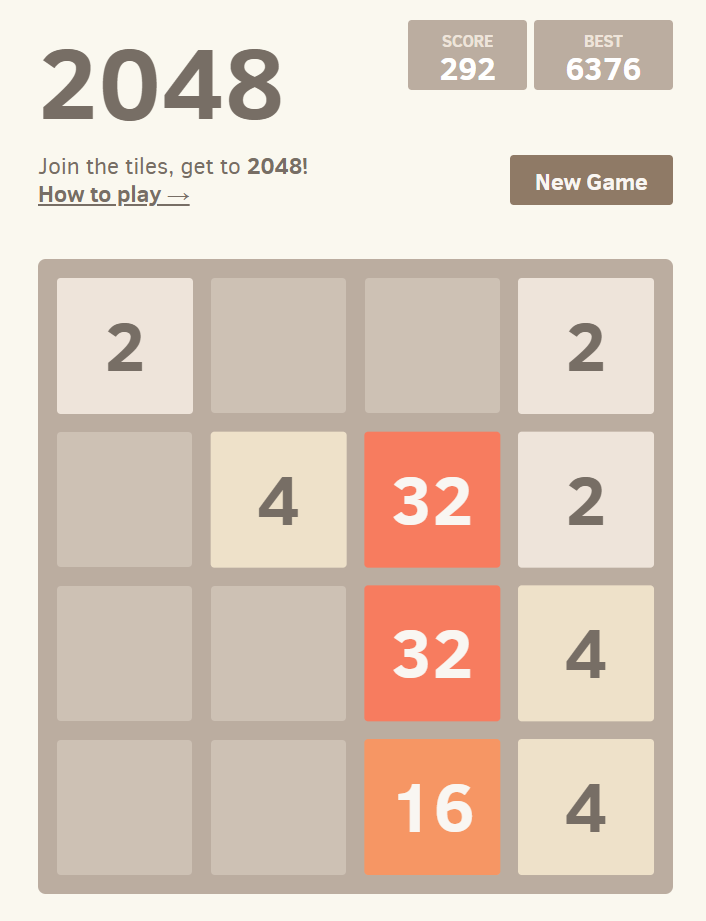
\includegraphics[width=0.45\textwidth]{Figures/2048.png}
  \caption{2048 \cite{2048}}
\end{figure}

\newpage

\section{Overview of the design}

This design applies Module View Specification (MVC) design pattern, Strategy design pattern and Singleton design pattern. The MVC components are \textit{GameController} (controller module), \textit{BoardT} (model module), and \textit{UserInterface} (view module) \cite{Bill}. For the Strategy design pattern, the \textit{EndCondition} (interface) captures the abstraction and the derived classes: \textit{EndByTime} and \textit{EndByMoves} encapsulate the implementation details. Singleton pattern is specified and implemented for \textit{GameController} and \textit{UserInterface}. 

\bigskip

\noindent An UML diagram is provided below for visualizing the structure of this software architecture \cite{UML}. 

\begin{figure}[hbt!]
  \centering
  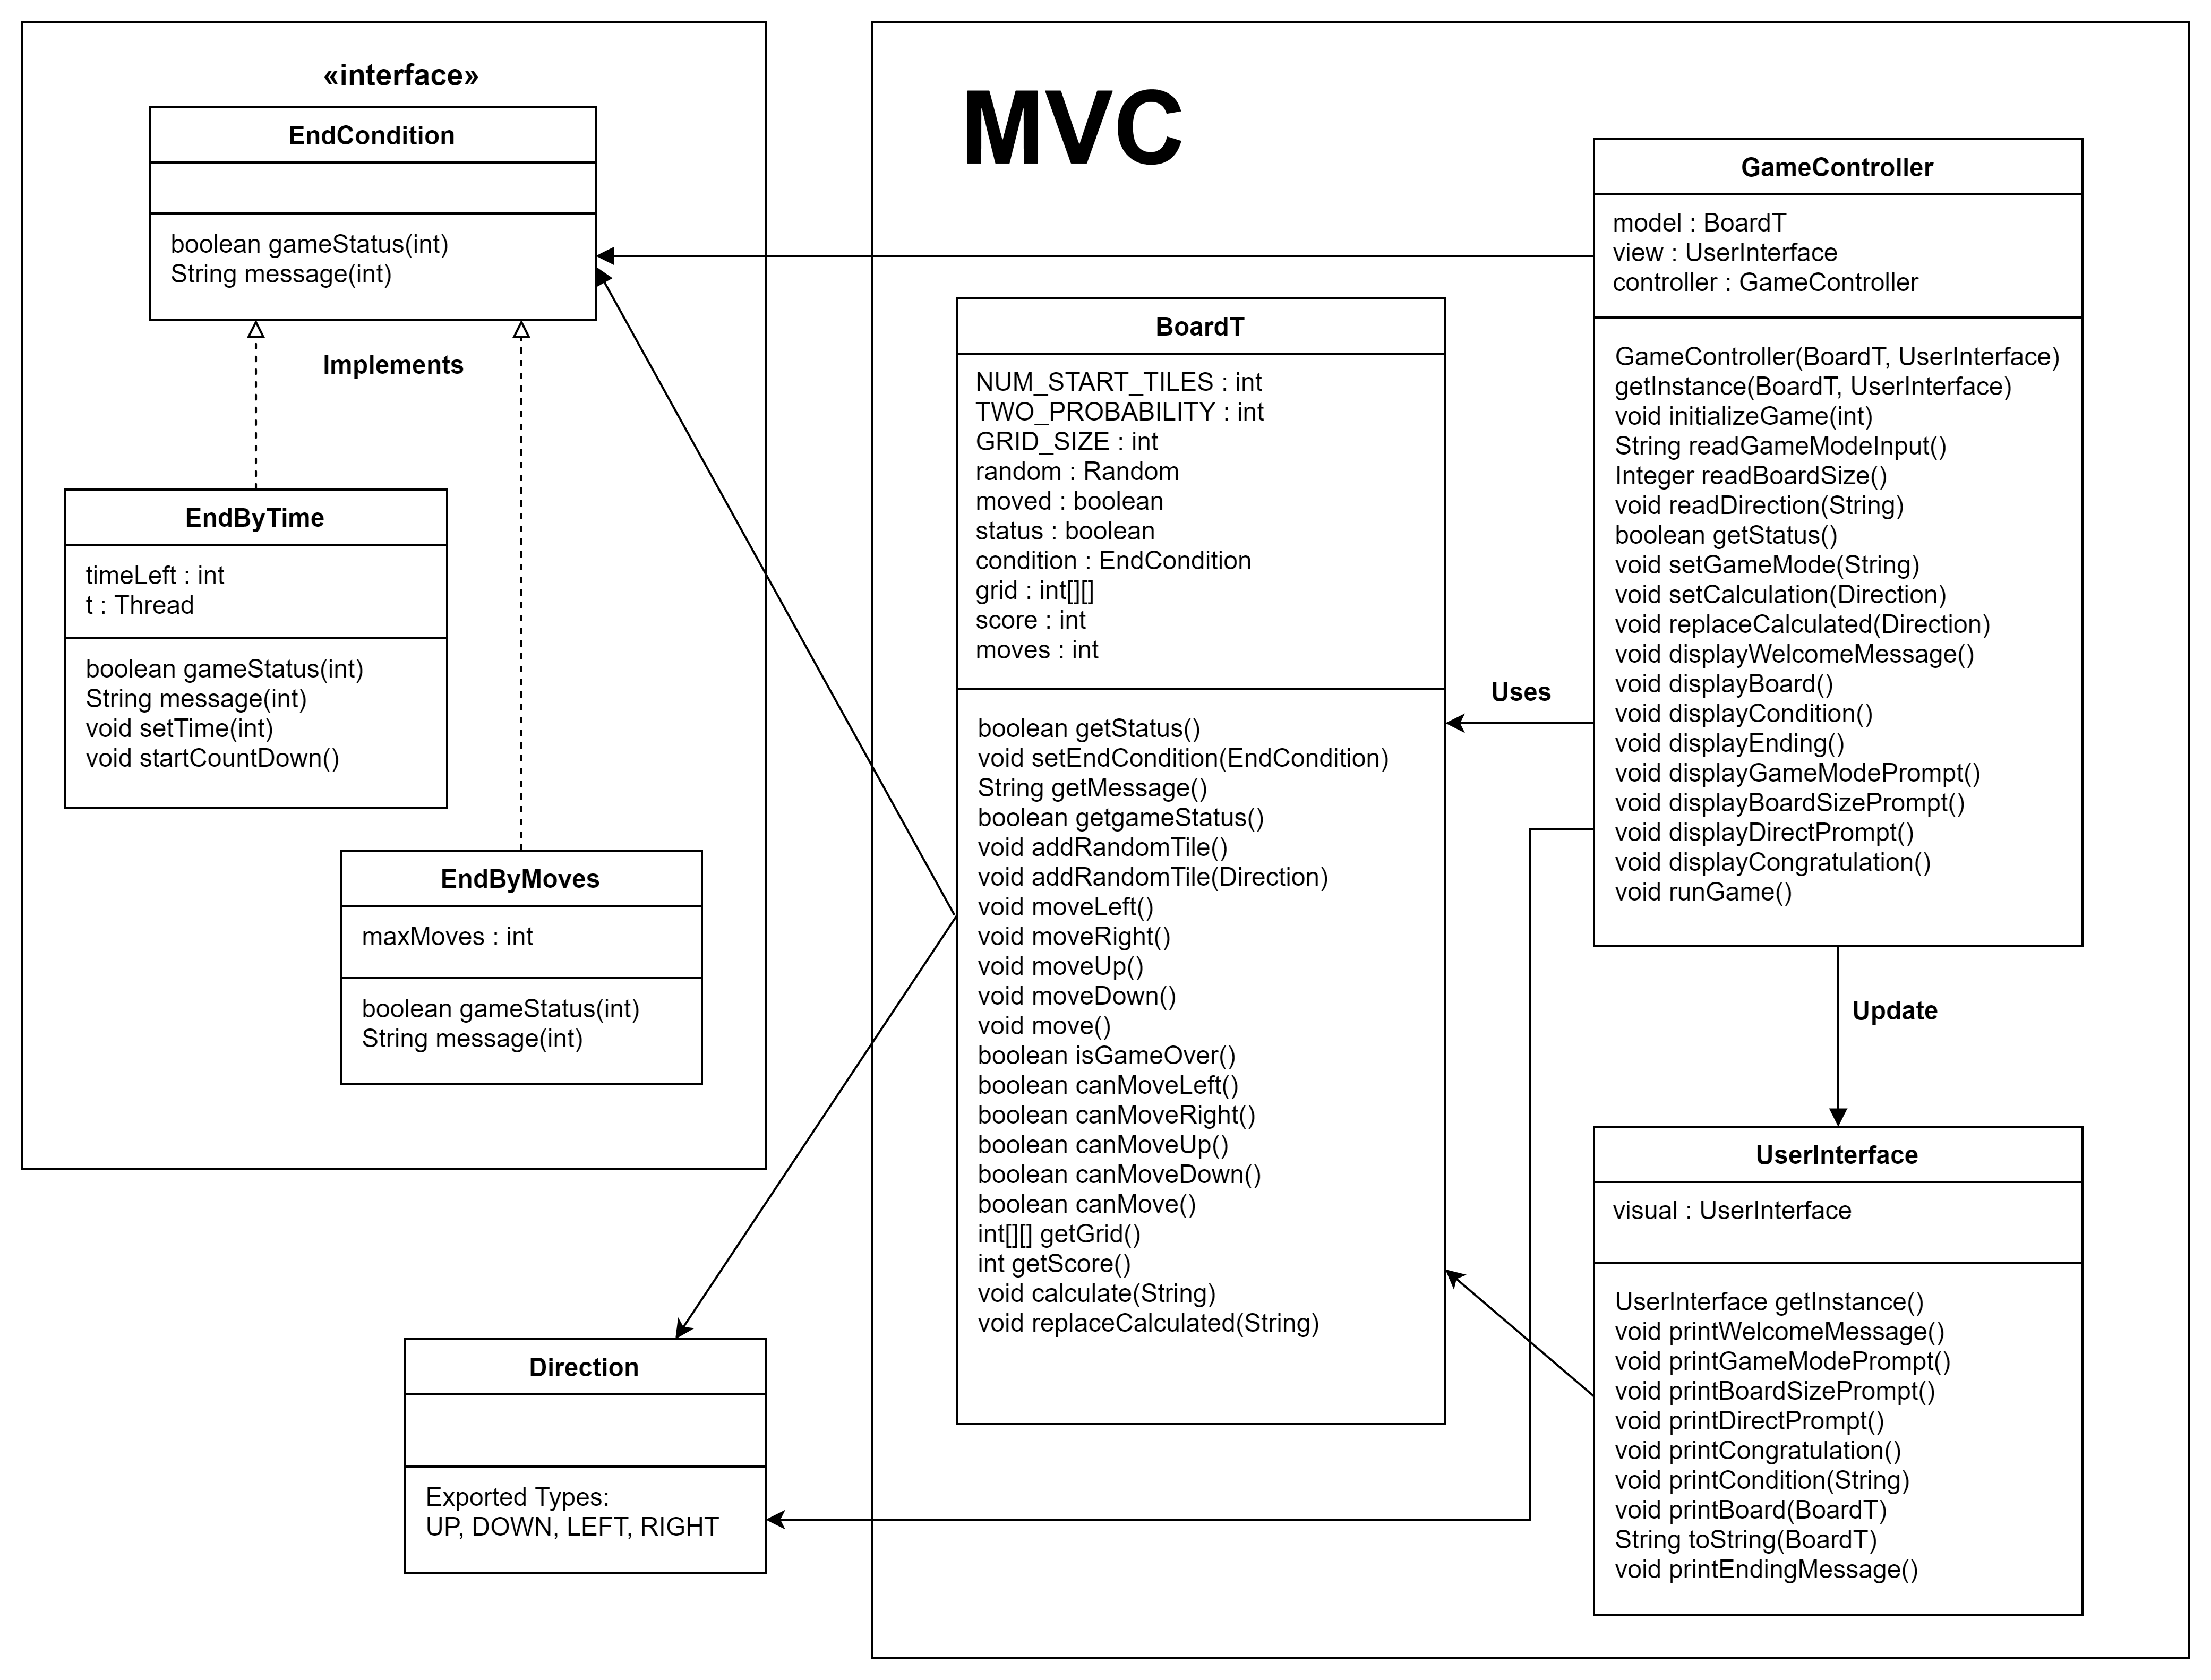
\includegraphics[width=1.0\textwidth]{Figures/UML.png}
  \caption{UML diagram of 2048}
\end{figure}

\newpage

\noindent The MVC design pattern is specified and implemented in the following way: the module \textit{BoardT}
stores the state of the game board and the status of the game. A view module \textit{UserInterface} can display
the state of the game board and game using a text-based graphics. The controller \textit{GameController}
is responsible for controlling the flow of the game by handling input actions, and interacting with the model and view modules.

\medskip

\noindent The implementation of the Strategy pattern enables the game ending condition to be changeable during
runtime. The user can choose the game mode to end the game after a time limit \textit{EndByTime} or after a specified amount of moves (\textit{EndByMoves}).

\medskip

\noindent For the Singleton design pattern, \textit{GameController} and \textit{UserInterface} use the \verb|getInstance()| method to obtain the abstract object.

\bigskip

\subsection*{Likely Changes my design considers:}

\begin{itemize}
  \item Data structure used for storing the game board
  \item The visual representation of the game such as UI layout. 
  \item Change in peripheral devices for taking user input. 
  \item Change in game ending conditions to adjust the difficulty of the game.
\end{itemize}

\newpage

\section* {Direction Module}

\subsection*{Module}

Direction

\subsection* {Uses}

N/A

\subsection* {Syntax}

\subsubsection* {Exported Constants}

None

\subsubsection* {Exported Types}

Direction = \{UP, DOWN, LEFT, RIGHT\}

\medskip

\subsubsection* {Exported Access Programs}

None

\subsection* {Semantics}

\subsubsection* {State Variables}

None

\subsubsection* {State Invariant}

None

\newpage

\section* {EndCondition Interface Module}

\subsection* {Interface Module}

EndCondition

\subsection*{Uses}

None

\subsection* {Syntax}

\subsubsection*{Exported Constants}

None

\subsubsection*{Exported Types}

None

\subsubsection* {Exported Access Programs}

\begin{tabular}{| l | l | l | p{6cm} |}
\hline
\textbf{Routine name} & \textbf{In} & \textbf{Out} & \textbf{Exceptions}\\
\hline
gameStatus & $\mathbb{N}$ & $\mathbb{B}$ & \\
\hline
message & $\mathbb{N}$ & $String$ & \\
\hline
\end{tabular}

\newpage

\section* {EndByMoves Module}

\subsection* {Template Module implements EndCondition Interface}

EndByMoves

\subsection*{Uses}

EndCondition

\subsection* {Syntax}

\subsubsection*{Exported Constants}

None

\subsubsection*{Exported Types}

None

\subsubsection* {Exported Access Programs}

\begin{tabular}{| l | l | l | p{6cm} |}
\hline
\textbf{Routine name} & \textbf{In} & \textbf{Out} & \textbf{Exceptions}\\
\hline
EndByMoves & ~ & EndByMoves & \\
\hline
\end{tabular}

\subsection* {Semantics}

\subsubsection*{State Variables}

maxMoves: $\mathbb{N}$ 

\subsubsection*{State Invariant}

None

\subsubsection*{Assumptions}

None

\subsubsection* {Access Routine Semantics}

new EndByMoves():

\begin{itemize}
  \item transition: maxMoves $:=$ 2048
  \item output: $out$ $:=$ self
  \item exception: none
\end{itemize}

\noindent gameStatus(moves):

\begin{itemize}
  \item output: $out$ $:=$ $\lnot$ ((maxMoves) - moves $<=$ 0)
  \item exception: none
\end{itemize}

\noindent message():
\begin{itemize}
  \item output: $out$ $:=$ A string containing information about the number of moves left
  \item exception: none
\end{itemize}

\newpage

\section* {EndByTime Module}

\subsection* {Template Module implements EndCondition Interface}

EndByTime

\subsection*{Uses}

EndCondition, Runnable

\subsection* {Syntax}

\subsubsection*{Exported Constants}

None

\subsubsection*{Exported Types}

None

\subsubsection* {Exported Access Programs}

\begin{tabular}{| l | l | l | p{6cm} |}
\hline
\textbf{Routine name} & \textbf{In} & \textbf{Out} & \textbf{Exceptions}\\
\hline
EndByTime & ~ & EndByTime    & \\
\hline
setTime & $\mathbb{N}$ & ~ & \\
\hline
startCountDown & ~ & ~ & \\
\hline
\end{tabular}

\subsection* {Semantics}

\subsubsection*{Environment Variables}

t: Thread

\subsubsection*{State Variables}

timeLeft: $\mathbb{N}$ \\

\subsubsection*{State Invariant}

None

\subsubsection*{Assumptions}

None

\subsubsection* {Access Routine Semantics}

new EndByTime():

\begin{itemize}
  \item output: $out$ $:=$ self
  \item transition: timeLeft, t $:=$ 600, new Thread(Run(this)) \\ \textit{// initiates the timer in thread t}
  \item exception: none
\end{itemize}

\noindent gameStatus(moves):

\begin{itemize}
  \item output: $\lnot$ (timeLeft $<=$ 0)
  \item exception: none
\end{itemize}

\noindent message(moves):
\begin{itemize}
  \item output: $out :=$ A string containing information about the time left
  \item exception: none
\end{itemize}

\noindent setTime(time):
\begin{itemize}
  \item transition: timeLeft $:=$ time
  \item output: none
  \item exception: none
\end{itemize}

\noindent startCountDown():
\begin{itemize}
  \item transition: t.start() \quad \textit{// Starts the count down clock in the thread}
  \item output: none
  \item exception: none
\end{itemize}


\newpage

\section* {BoardT ADT Module}

\subsection*{Template Module}

BoardT

\subsection* {Uses}

EndCondition, Direction

\subsection* {Syntax}

\subsubsection* {Exported Types}

None

\subsubsection* {Exported Constant}

None

\subsubsection* {Exported Access Programs}

\begin{tabular}{| l | l | l | l |}
\hline
\textbf{Routine name} & \textbf{In} & \textbf{Out} & \textbf{Exceptions}\\
\hline
BoardT & $\mathbb{N}$, Random & BoardT & \\
\hline
getStatus & ~ & $\mathbb{B}$ & \\
\hline
setEndCondition & EndCondition &  & \\
\hline
getMessage & ~ & String & \\
\hline
getgameStatus &  & String & \\
\hline
addRandomTile &  &  & \\
\hline
addRandomTile  &  Direction  &  & \\
\hline
move  & Direction  & $\mathbb{B}$ & \\
\hline
isGameOver  &   & $\mathbb{B}$ & \\
\hline
canMove  & Direction  &  $\mathbb{B}$ & \\
\hline
getGrid  &  &  seq of (seq of $\mathbb{N}$) & \\
\hline
getScore  &  &  $\mathbb{N}$ & \\
\hline
\end{tabular}

\subsection* {Semantics}

\subsubsection* {State Variables}

NUM\_START\_TILES: $\mathbb{N}$ \\
TWO\_PROBABILITY: $\mathbb{N}$ \\
GRID\_SIZE: $\mathbb{N}$\\
random: Random\\
moved: $\mathbb{B}$\\
status: $\mathbb{B}$\\
condition: EndCondition\\
grid: sequence of (sequence of $\mathbb{N}$)\\
score: $\mathbb{N}$\\
moves: $\mathbb{N}$\\

\subsubsection* {State Invariant}

None

\subsubsection* {Assumptions}

\begin{itemize}
  \item The constructor BoardT is called for each object instance before any other access routine 
  is called for that object. 
  \item Assume there is a random function that generates a random value beteern 0 and 1.
  \item Players can choose the board size from 1 to infinite.
  \item Players can choose the game mode which are ``limited moves mode'' and ``limited time mode''.
  \item If there is a way for blocks to be added, the game continues, otherwise the game ends.
  \item If the board has more than 30\% empty position, a new block is created at a random position. 
  \item When the grid size is bigger than 6 and there are more than 30\% empty places, then the number of created blocks increased by boardsize - 4.
  \item Block 2 is created with a possibility of 90\%, and block 4 is created with a possiblity of 10\%. 
  \item When the game score reaches 2048, print ``Congratulation'' message and continue the game.
\end{itemize}

\subsubsection* {Design decision}

Players can choose the size of the board and game mode which are ``limited moves mode'' and ``limited time mode''. When the board size is 1 there is no place to move, so it ends automatically. Players can choose any size of board but for the simplicity of implementation, the game mode's limit condition doesn't change. For example, it the ``limited moves mode'', the max\_movement is 2048, and in the ``limited time mode'', the limited time is 600s. 

\subsubsection* {Access Routine Semantics}

BoardT(boardSize, random):
\begin{itemize}
\item transition: \\
      random $:=$ random\\
      GRID\_SIZE $:=$ boardSize\\
      grid $:=$ $ \langle t :$ Seq of Integer $|$ $t_{i} \wedge i \in [0..|boardSize|-1] : |t| = |boardSize| \rangle $\\
      score, moves, status $:=$ 0, 0, true
\item output: $out$ $:=$ self
\item exception: none
\end{itemize}

\noindent getStatus():
\begin{itemize}
\item output: $out :=$ status
\item exception: none
\end{itemize}

\noindent setEndCondition(condition):
\begin{itemize}
\item transition: condition $:=$ condition
\item output: none 
\item exception: none
\end{itemize}

\noindent getMessage():
\begin{itemize}
\item output: $out :=$ (condtion.message(moves))
\item exception: none
\end{itemize}

\noindent getgameStatus():
\begin{itemize}
\item output: $out :=$ condition.gameStatus(moves)
\item exception: none
\end{itemize}

\noindent addRandomTile():
\begin{itemize}
\item output: grid $:=$ ($\exists i, j, k, l \in \mathbb{N}$ $|$ $i, j, k, l < |boardSize|-1 : grid[i][j] := 2 \wedge grid[k][j] := 2$)
\item exception: none
\end{itemize}

\noindent addRandomTile(direction):
\begin{itemize}
\item transition: grid $:=$ canMove(direction) $\Rightarrow$ ($\exists i, j \in \mathbb{N}$ $|$ $i, j < |boardSize|-1 : grid[i][j] := 2 \vee grid[i][j] := 4$)
\item output: none
\item exception: none
\end{itemize}

\noindent move(direction):
\begin{itemize}
\item output: $out :=$ ((direction = Direction.LEFT $\Rightarrow$ moveLeft()) $||$ (direction = Direction.RIGHT $\Rightarrow$ moveRight()) $||$ (direction = Direction.UP $\Rightarrow$ moveUp()) $||$ (direction = Direction.DOWN $\Rightarrow$ moveDown()))  
\item exception: none
\end{itemize}

\noindent isGameOver():
\begin{itemize}
\item output: $out :=$ ($\lnot$(canMoveLeft()) $\wedge$ $\lnot$(canMoveRight()) $\wedge$ $\lnot$(canMoveUp()) $\wedge$ $\lnot$(canMoveDown()))
\item exception: none
\end{itemize}

\noindent canMove(direction):
\begin{itemize}
\item output: $out :=$ ((direction = Direction.LEFT $\wedge$ canMoveLeft()) $||$ (direction = Direction.RIGHT $\wedge$ canMoveRight()) $||$ (direction = Direction.UP $\wedge$ canMoveUp()) $||$(direction = Direction.DOWN $\wedge$ canMoveDown()))  
\item exception: none
\end{itemize}

\noindent getGrid():
\begin{itemize}
\item output: $out :=$ grid  
\item exception: none
\end{itemize}

\noindent getScore():
\begin{itemize}
\item output: $out :=$ score  
\item exception: none
\end{itemize}

\subsubsection* {Local Functions}

\noindent moveLeft: void $\rightarrow$ void \\
moveLeft $\equiv$ ($\exists i, j \in \mathbb{N}$ $|$ $i,j < |boardSize|-1$ : $grid[i][j-1]=0 \wedge \lnot (grid[i][j]=0) \Rightarrow grid[i][j-1] := grid[i][j] \wedge grid[i][j]:=0$) $\wedge$ ($\exists i, j \in \mathbb{N}$ $|$ $i,j < |boardSize|-1$ : $(grid[i][j-1] = grid[i][j]) \Rightarrow grid[i][j-1] := grid[i][j-1] + grid[i][j] \wedge grid[i][j]:=0$)\\

\noindent moveRight: void $\rightarrow$ void \\
moveRight $\equiv$ ($\exists i, j \in \mathbb{N}$ $|$ $i,j < |boardSize|-1$ : ($\lnot (grid[i][j-1]=0) \wedge grid[i][j]=0 \Rightarrow grid[i][j] := grid[i][j-1] \wedge grid[i][j-1]:=0$) $\wedge$ ($\exists i, j \in \mathbb{N}$ $|$ $i,j < |boardSize|-1$ : $(grid[i][j-1] = grid[i][j]) \Rightarrow grid[i][j] := grid[i][j-1] + grid[i][j] \wedge grid[i][j-1]:=0$)\\

\noindent moveUp: void $\rightarrow$ void \\
moveUp $\equiv$ ($\exists i, j \in \mathbb{N}$ $|$ $i,j < |boardSize|-1$ : ($grid[i-1][j]=0 \wedge \lnot(grid[i][j]=0) \Rightarrow grid[i-1][j] := grid[i][j] \wedge grid[i][j]:=0$) $\wedge$ ($\exists i, j \in \mathbb{N}$ $|$ $i,j < |boardSize|-1$ : $(grid[i-1][j] = grid[i][j]) \Rightarrow grid[i-1][j] := grid[i-1][j] + grid[i][j] \wedge grid[i][j]:=0$)\\

\noindent moveDown: void $\rightarrow$ void \\
moveDown $\equiv$ ($\exists i, j \in \mathbb{N}$ $|$ $i,j < |boardSize|-1$ : ($\lnot (grid[i-1][j]=0) \wedge grid[i][j]=0 \Rightarrow grid[i][j] := grid[i-1][j] \wedge grid[i-1][j]:=0$) $\wedge$ ($\exists i, j \in \mathbb{N}$ $|$ $i,j < |boardSize|-1$ : $(grid[i-1][j] = grid[i][j]) \Rightarrow grid[i][j] := grid[i-1][j] + grid[i][j] \wedge grid[i-1][j]:=0$)\\

\noindent canMoveLeft: void $\rightarrow \mathbb{B}$  \\
canMoveLeft $\equiv$ ($\exists i, j \in \mathbb{N}$ $|$ $i,j < |boardSize|-1$ : $(grid[i][j-1]=0 \wedge \lnot(grid[i][j]=0)) \vee (\lnot(grid[i][j-1]=0) \wedge grid[i-1][j]=grid[i][j]$))\\

\noindent canMoveRight: void $\rightarrow \mathbb{B}$  \\
canMoveRight $\equiv$ ($\exists i, j \in \mathbb{N}$ $|$ $i,j < |boardSize|-1$ : $(\lnot(grid[i][j-1]=0) \wedge (grid[i][j]=0)) \vee (\lnot(grid[i][j-1]=0) \wedge grid[i][j-1]=grid[i][j]$))\\

\noindent canMoveUp: void $\rightarrow \mathbb{B}$  \\
canMoveUp $\equiv$ ($\exists i, j \in \mathbb{N}$ $|$ $i,j < |boardSize|-1$ : $(grid[i-1][j]=0 \wedge \lnot(grid[i][j]=0)) \vee (\lnot(grid[i-1][j]=0) \wedge grid[i-1][j]=grid[i][j]$))\\

\noindent canMoveDown: void $\rightarrow \mathbb{B}$  \\
canMoveDown $\equiv$ ($\exists i, j \in \mathbb{N}$ $|$ $i,j < |boardSize|-1$ : $(\lnot(grid[i-1][j]=0) \wedge grid[i][j]=0) \vee (\lnot(grid[i-1][j]=0) \wedge grid[i-1][j]=grid[i][j]$))\\

\medskip

\newpage

\section* {UserInterface Module (Abstract Object)}

\subsection* {Module}

UserInterface

\subsection* {Uses}

BoardT

\subsection* {Syntax}

\subsubsection* {Exported Types}

None

\subsubsection* {Exported Constants}

None

\subsubsection* {Exported Access Programs}

\begin{tabular}{| l | l | l | p{6cm} |}
\hline
\textbf{Routine name} & \textbf{In} & \textbf{Out} & \textbf{Exceptions}\\
\hline
getInstance & ~ & UserInterface &  \\
\hline
printWelcomeMessage & ~ & ~ & \\
\hline
printGameModePrompt & ~ & ~ & \\
\hline
printBoardSizePrompt & ~ & ~ & \\
\hline
printDirectPrompt & String & ~ & \\
\hline
printCongratulation & String & ~ & \\
\hline
printCondition & String & ~ & \\
\hline
printBoard & String & ~ & \\
\hline
printEndingMessage & ~ & ~ & \\
\hline
\end{tabular}

\subsection* {Semantics}

\subsubsection*{Environment Variables}

None

\subsubsection* {State Variables}

visual: UserInterface

\subsubsection* {State Invariant}

None

\subsubsection* {Assumptions}

\begin{itemize}
\item The UserInterface constructor is called for each object instance before any
other access routine is called for that object.  The constructor can only be
called once.
\end{itemize}

\subsubsection* {Access Routine Semantics}

\noindent getInstance():
\begin{itemize}
  \item transition: visual $:=$ (visual = null $\Rightarrow$ new UserInterface())
  \item output: $out$ $:=$ self
  \item exception: none
\end{itemize}

\noindent printWelcomeMessage():
\begin{itemize}
  \item output: none
  \item exception: none
\end{itemize}

\noindent printGameModePrompt():
\begin{itemize}
  \item output: none
  \item exception: none
\end{itemize}

\noindent printBoardSizePrompt():
\begin{itemize}
  \item output: none
  \item exception: none
\end{itemize}

\noindent printDirectPrompt():
\begin{itemize}
  \item output: none
  \item exception: none
\end{itemize}

\noindent printCongratulation():
\begin{itemize}
  \item output: none
  \item exception: none
\end{itemize}

\noindent printCondition(message):
\begin{itemize}
  \item output: none  //Print the message
  \item exception: none
\end{itemize}

\noindent printBoardT(boardT):
\begin{itemize}
  \item output: none  //Print toString(boardT)
  \item exception: none
\end{itemize}

\noindent printEndingMessage(boardT):
\begin{itemize}
  \item output: none
  \item exception: none
\end{itemize}

\subsubsection*{Local Function:}

\noindent UserInterface: void $\rightarrow$ UserInterface \\
UserInterface() $\equiv$ new UserInterface()\\

\noindent toString: BoardT $\rightarrow$ String
toString(boardT) $\equiv$ Print grid information

\newpage

\section* {GameController Module (Abstract Object)}

\subsection* {Module}

GameController

\subsection* {Uses}

BoardT, UserInterface

\subsection* {Syntax}

\subsubsection* {Exported Types}

None

\subsubsection* {Exported Constants}

None

\subsubsection* {Exported Access Programs}

\begin{tabular}{| l | l | l | p{4.7cm} |}
\hline
\textbf{Routine name} & \textbf{In} & \textbf{Out} & \textbf{Exceptions}\\
\hline
getInstance & BoardT, UserInterface & GameController & ~ \\
\hline
initializeGame & $\mathbb{N}$ & ~ & ~\\
\hline
readGameModeInput & String & ~ & IllegalArgumentException \\
\hline
readBoardSize & $\mathbb{N}$ & ~ & IllegalArgumentException \\
\hline
readDirection& String & Direction & IllegalArgumentException \\
\hline
getStatus& ~ & $\mathbb{B}$ & ~ \\
\hline
getGameMode& String & ~ & ~ \\
\hline
setCalculation& Direciton & ~ & ~ \\
\hline
replaceCalculated& Direction & ~ & ~ \\
\hline
displayWelcomeMessage& ~ & ~ & ~ \\
\hline
displayBoard& ~ & ~ & ~ \\
\hline
displayCondition& ~ & ~ & ~ \\
\hline
displayEnding& ~ & ~ & ~ \\
\hline
displayGameModePrompt& ~ & ~ & ~ \\
\hline
displayBoardSizePrompt& ~ & ~ & ~ \\
\hline
displayDirectPrompt& ~ & ~ & ~ \\
\hline
displayCongratulation& ~ & ~ & ~ \\
\hline
runGame & ~ & ~ & ~ \\
\hline
\end{tabular}

\subsection* {Semantics}

\subsubsection*{Environment Variables}

keyboard: Scanner(System.in) \qquad \textit{// reading inputs from keyboard}

\subsubsection* {State Variables}

model: BoardT \\
view: UserInterface \\
controller: GameController

\subsubsection* {State Invariant}

None

\subsubsection* {Assumptions}

\begin{itemize}
  \item The GameController constructor is called for each object instance before any
  other access routine is called for that object.  The constructor can only be
  called once.
  \item Assume that model and view instances are already initialized before calling GameController
        constructor
\end{itemize}

\subsubsection* {Access Routine Semantics}

\noindent getInstance(model, view):
\begin{itemize}
  \item transition: controller $:=$ (controller = null $\Rightarrow$ new GameController (model, view))
  \item output: $out$ $:=$ self
  \item exception: none
\end{itemize}

\noindent initializeGame(boardSize):
\begin{itemize}
  \item transition: model $:=$ new BoardT(boardSize, new Random())
  \item output: none
  \item exception: none
\end{itemize}

\noindent readGameModeInput():
\begin{itemize}
  \item output: $out$ $:=$ gameMode $=$ input from an user by the keyboard
  \item exception: $exc$ $:=$ ($(gamemode \neq m) \wedge (gamemode \neq t) \wedge (gamemode \neq e)$) $\Rightarrow$ IllegalArgumentException\\
  // ``m'' limited moves mode, ``t'' limited time mode, ``e'' to exit the game
\end{itemize}

\noindent readBoardSize():
\begin{itemize}
  \item output: $out$ $:=$ boardsize $=$ input from an user by the keyboard
  \item exception: $exc$ $:=$ ($boardsize \leq 0) \Rightarrow$ IllegalArgumentException
\end{itemize}

\noindent readDirection(input):
\begin{itemize}
  \item output: $out$ $:=$ direction $=$ (input from an user by the keyboard) $\wedge$ ((input$=$Direction.UP $Rightarrow$ input $:=$ Direction.UP) $\vee$ (input$=$w $Rightarrow$ input $:=$ Direction.UP) $\vee$ (input$=$s $Rightarrow$ input $:=$ Direction.DOWN) $\vee$ (input$=$a $Rightarrow$ input $:=$ Direction.LEFT) $\vee$ (input$=$d $Rightarrow$ input $:=$ Direction.RIGHT))
  \item exception: $exc$ $:=$ ($(direction \neq w) \wedge (direction \neq s) \wedge (direction \neq a) \wedge (direction \neq d))$ $\Rightarrow$ IllegalArgumentException
\end{itemize}

\noindent getStatus():
\begin{itemize}
  \item output: $out$ $:=$ (model.getStatus())
  \item exception: none
\end{itemize}

\noindent setGameMode(input):
\begin{itemize}
  \item transition: model $:=$ (input $=$ m $\Rightarrow$ model.setEndCondition(new EndByMoves()) $\vee$ input $=$ t $\Rightarrow$ (condition $:=$ new EndByTime() $\wedge$ model.setEndCondition(condition) $\wedge$ condition.setCountDown())
  \item output: none
  \item exception: $exc$ $:=$ ($(input \neq m) \wedge (input \neq t)$) $\Rightarrow$ IllegalArgumentException
\end{itemize}

\noindent setCalculation(direction):
\begin{itemize}
  \item transition: model $:=$ model.move(direction)
  \item output: none
  \item exception: none
\end{itemize}

\noindent replaceCalculated(direction):
\begin{itemize}
  \item transition: model $:=$ model.addRandomTile(direction)
  \item output: none
  \item exception: none
\end{itemize}

\noindent displayWelcomeMessage():
\begin{itemize}
  \item transition: view $:=$ view.printWelcomeMessage()
  \item output: none
  \item exception: none
\end{itemize}

\noindent displayBoard():
\begin{itemize}
  \item transition: view $:=$ view.printBoard(model)
  \item output: none
  \item exception: none
\end{itemize}

\noindent displayCondition():
\begin{itemize}
  \item transition: view $:=$ view.printCondition(model.getMessage())
  \item output: none
  \item exception: none
\end{itemize}

\noindent displayEnding():
\begin{itemize}
  \item transition: view $:=$ view.printEndingMessage()
  \item output: none
  \item exception: none
\end{itemize}

\noindent displayGameModePrompt():
\begin{itemize}
  \item transition: view $:=$ view.printGameModePrompt()
  \item output: none
  \item exception: none
\end{itemize}

\noindent displayBoardSizePrompt():
\begin{itemize}
  \item transition: view $:=$ view.printBoardSizePrompt()
  \item output: none
  \item exception: none
\end{itemize}

\noindent displayDirectPrompt():
\begin{itemize}
  \item transition: view $:=$ view.printDirectPrompt()
  \item output: none
  \item exception: none
\end{itemize}

\noindent displayCongratulation():
\begin{itemize}
  \item transition: view $:=$ view.printCongratulation()
  \item output: none
  \item exception: none
\end{itemize}

\noindent runGame():
\begin{itemize}
  \item transition: operational method for running the game. The game will start with a welcome message, next asking the user to select a game mode, then display the board and let the user to play the game. Eventually, when the game ends, display the ending message.
  \item output: None
\end{itemize}

\subsubsection*{Local Function:}

GameController: BoardT $\times$ UserInterface $\rightarrow$ GameController \\
GameController($model, view$) $\equiv$ new GameController($model, view$)

\newpage

\section*{Critique of Design}

\begin{itemize}
  \item First of all, I referred to the previous year's assignment4 (two-dots), written by ``Bill Song''. Because ``two-dots'' and ``2048'' have a similiar software architecture, utlizing the proven design patterens can be a safe and efficient strategy. I took the advantageous design patterns from it such as Model View Specification, Strategy design pattern and Singleton design pattern. 
  \item MVC consists of three components, which are ``controller'', ``model'', and ``view''. Each component has a role such as \textit{controller} handles input actions, \textit{view} displays the data from the model component, and \textit{model} encapsulates system's data as well as operations on the data. As MVC components have their own roles, we can separate concerns increasing the maintainability and decreaseing risks about changes. MVC also keeps high cohesion since it groups related functionalities within each module. The deisgn is also low coupling because the modules (model, view, controller) are mostly independent of each other. So, a change in one of the modules does not heavily impact the other. However in oder to maintain high cohesion, I implemented the \verb|printBoard| method in UserInterface module (\textit{view}), which increases the coupling because I had to use BoardT module (\textit{model}).
  \item Strategy design pattern provides convenience and flexibility in designing for change. For example, this program applies strategy design pattern making the interface of \textit{EndCondition} with two options such as \textit{EndByTime} and \textit{EndByMoves}. This makes it easier to switch between different algorithms during runtime through polymorphism. In addition, it increases maintainability and readability in a way that the concerns are separated into classes instead of using conditional statements to switch strategy in runtime.
  \item Singleton design pattern ensures that a class has only one instance and provides a global point of access to that instance. Because it has only one instance, we can decrease the potential conflicts in the software which incerases the reliability. For instance, as one GameController instance handles all inputs and communicates with the one UserInterface instance, we can significantly increase the clarity, verifiability, and reduce the ambiguity of software.
  \item I made the game more general by allowing users can choose the board size. However, when the board size is 1, there is no place to move, so the game will end right away. I also set that when the grid size is bigger than 6 and there are more than 70\% empty places, then the number of created blocks increased by boardsize - 4. And I increased the usability after reflecting a real feedback from a user(my brother), I changed the input keys from ``U, D, L, R'' to ``w, s, a, d''.
  \item When I checked the MIS, I found that the terms of board and grid were used for the same meaning. Thus we can say that this is not consistent.
  \item We can also see the information hiding in the interface module(\textit{EndCondition}) and its implementations protecting other parts of the program from extensive modification. And as I mentioned in the MVC design pattern, it has high cohesion because each components of MVC are highly related to each others.
  \item We can also check it's not essential because I implemented \verb|addRandomTile()| method two times in BoardT, with and without parameter for the simplicity of the implementation and readability of the code. But I was able to implement it in a same method by using a conditional sentence.
  \item As we can see in the \textit{moveUp}, \textit{moveDown}, \textit{moveLeft}, \textit{moveRight}, and \textit{move} methods, each method has only one role. So, we can say it's minimal.
  \item Because the game states change randomly according to the input of the user, testing all methods automatically was impossible. I made $AllTests.java$ file for testing $TestBoardT.java$, $TestEndByMoves.java$, and $TestEndByTime.java$. Except for some methods which are possible to test automatically, I verified and tested the software incrementally. Whenever there are small changes, I tested them. You can run the game with the Demo.java file and also ``make expt'' command on mills. The test cases are designed to validate the correctness of the program based on the requirement and reveal errors or unusual behavior during program execution, every access routine has at least one test case. 
\end{itemize}

\newpage

\section*{Answers to Questions:}

Q1: UML diagram for the modules in A3.\\
\begin{itemize}
  \item Abstrac Data Types : AttributeT, CourseT, LOsT, ProgramT(subclass), IndicatorT(enum), HashSet(generic)
  \item Module : Measures(Interface)
  \item Abstract Objects : Norm
  \item Libraries : Services
\end{itemize}

\begin{figure}[h!]
  \centering
  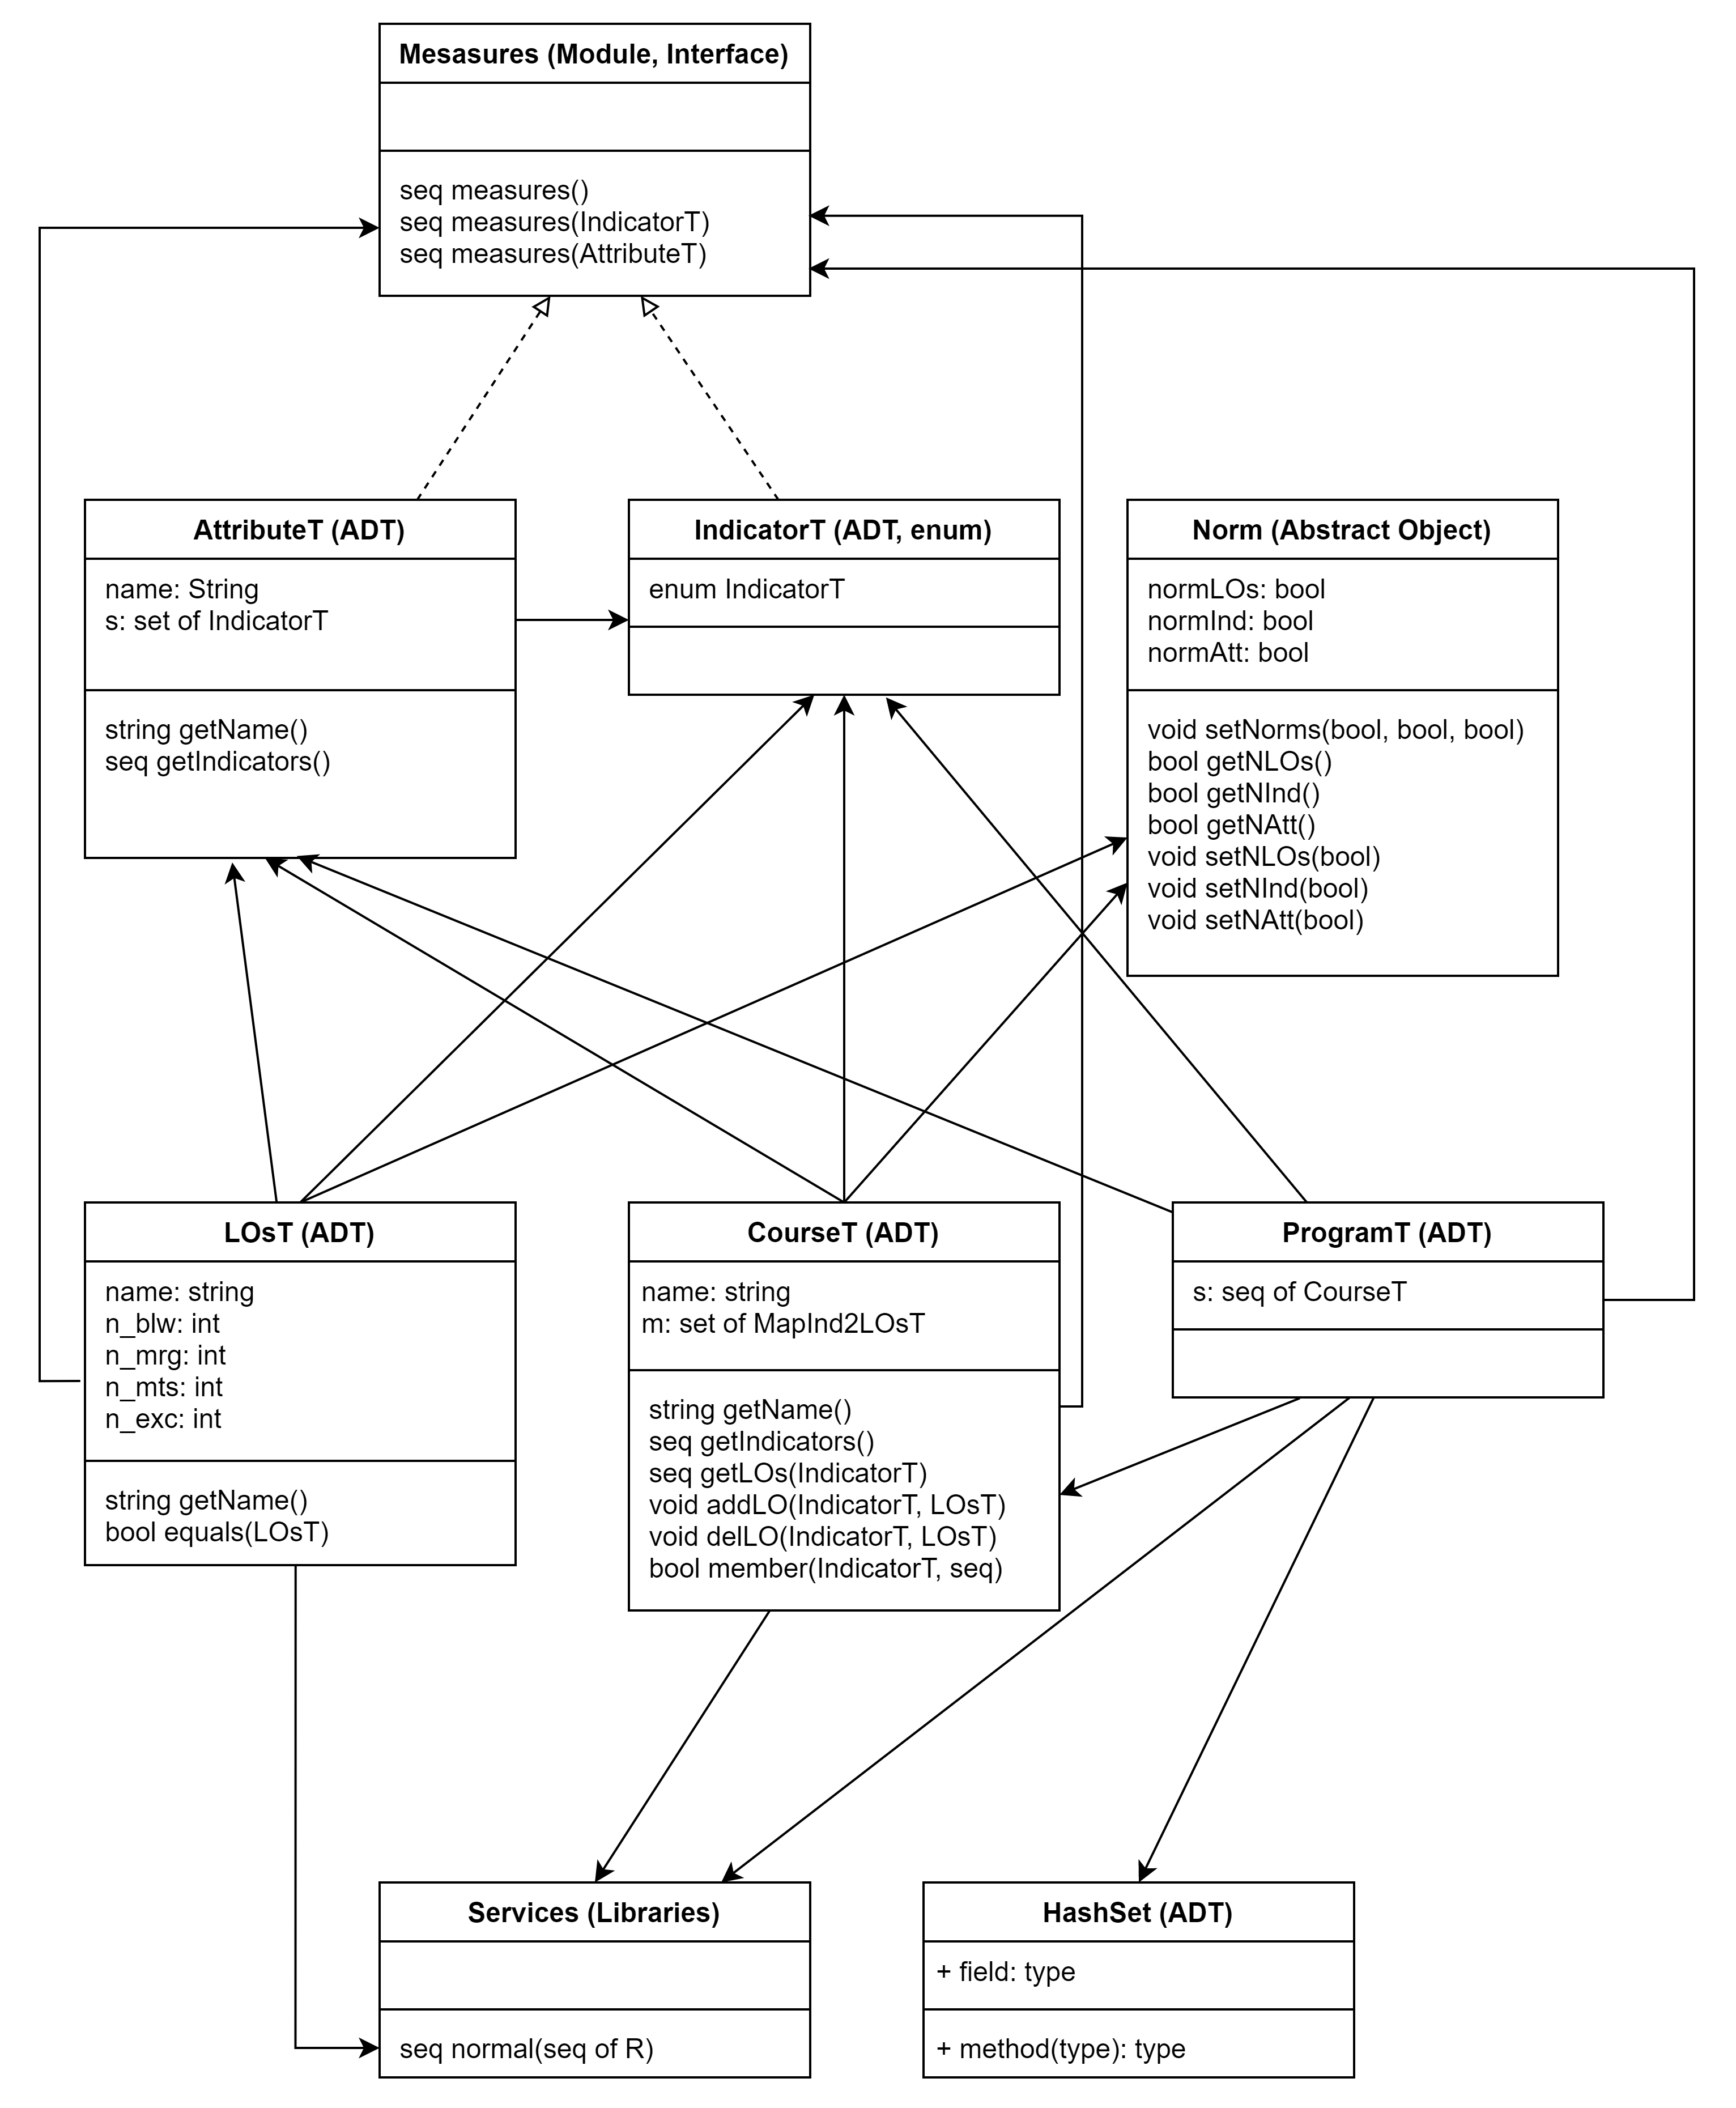
\includegraphics[width=0.9\textwidth]{Figures/A3UML.png}
  \caption{Question 1. UML diagram of A3}
\end{figure}

\medskip

\noindent Q2:  Draw a control flow graph for the convex hull algorithm.\\

\begin{figure}[h!]
  \centering
  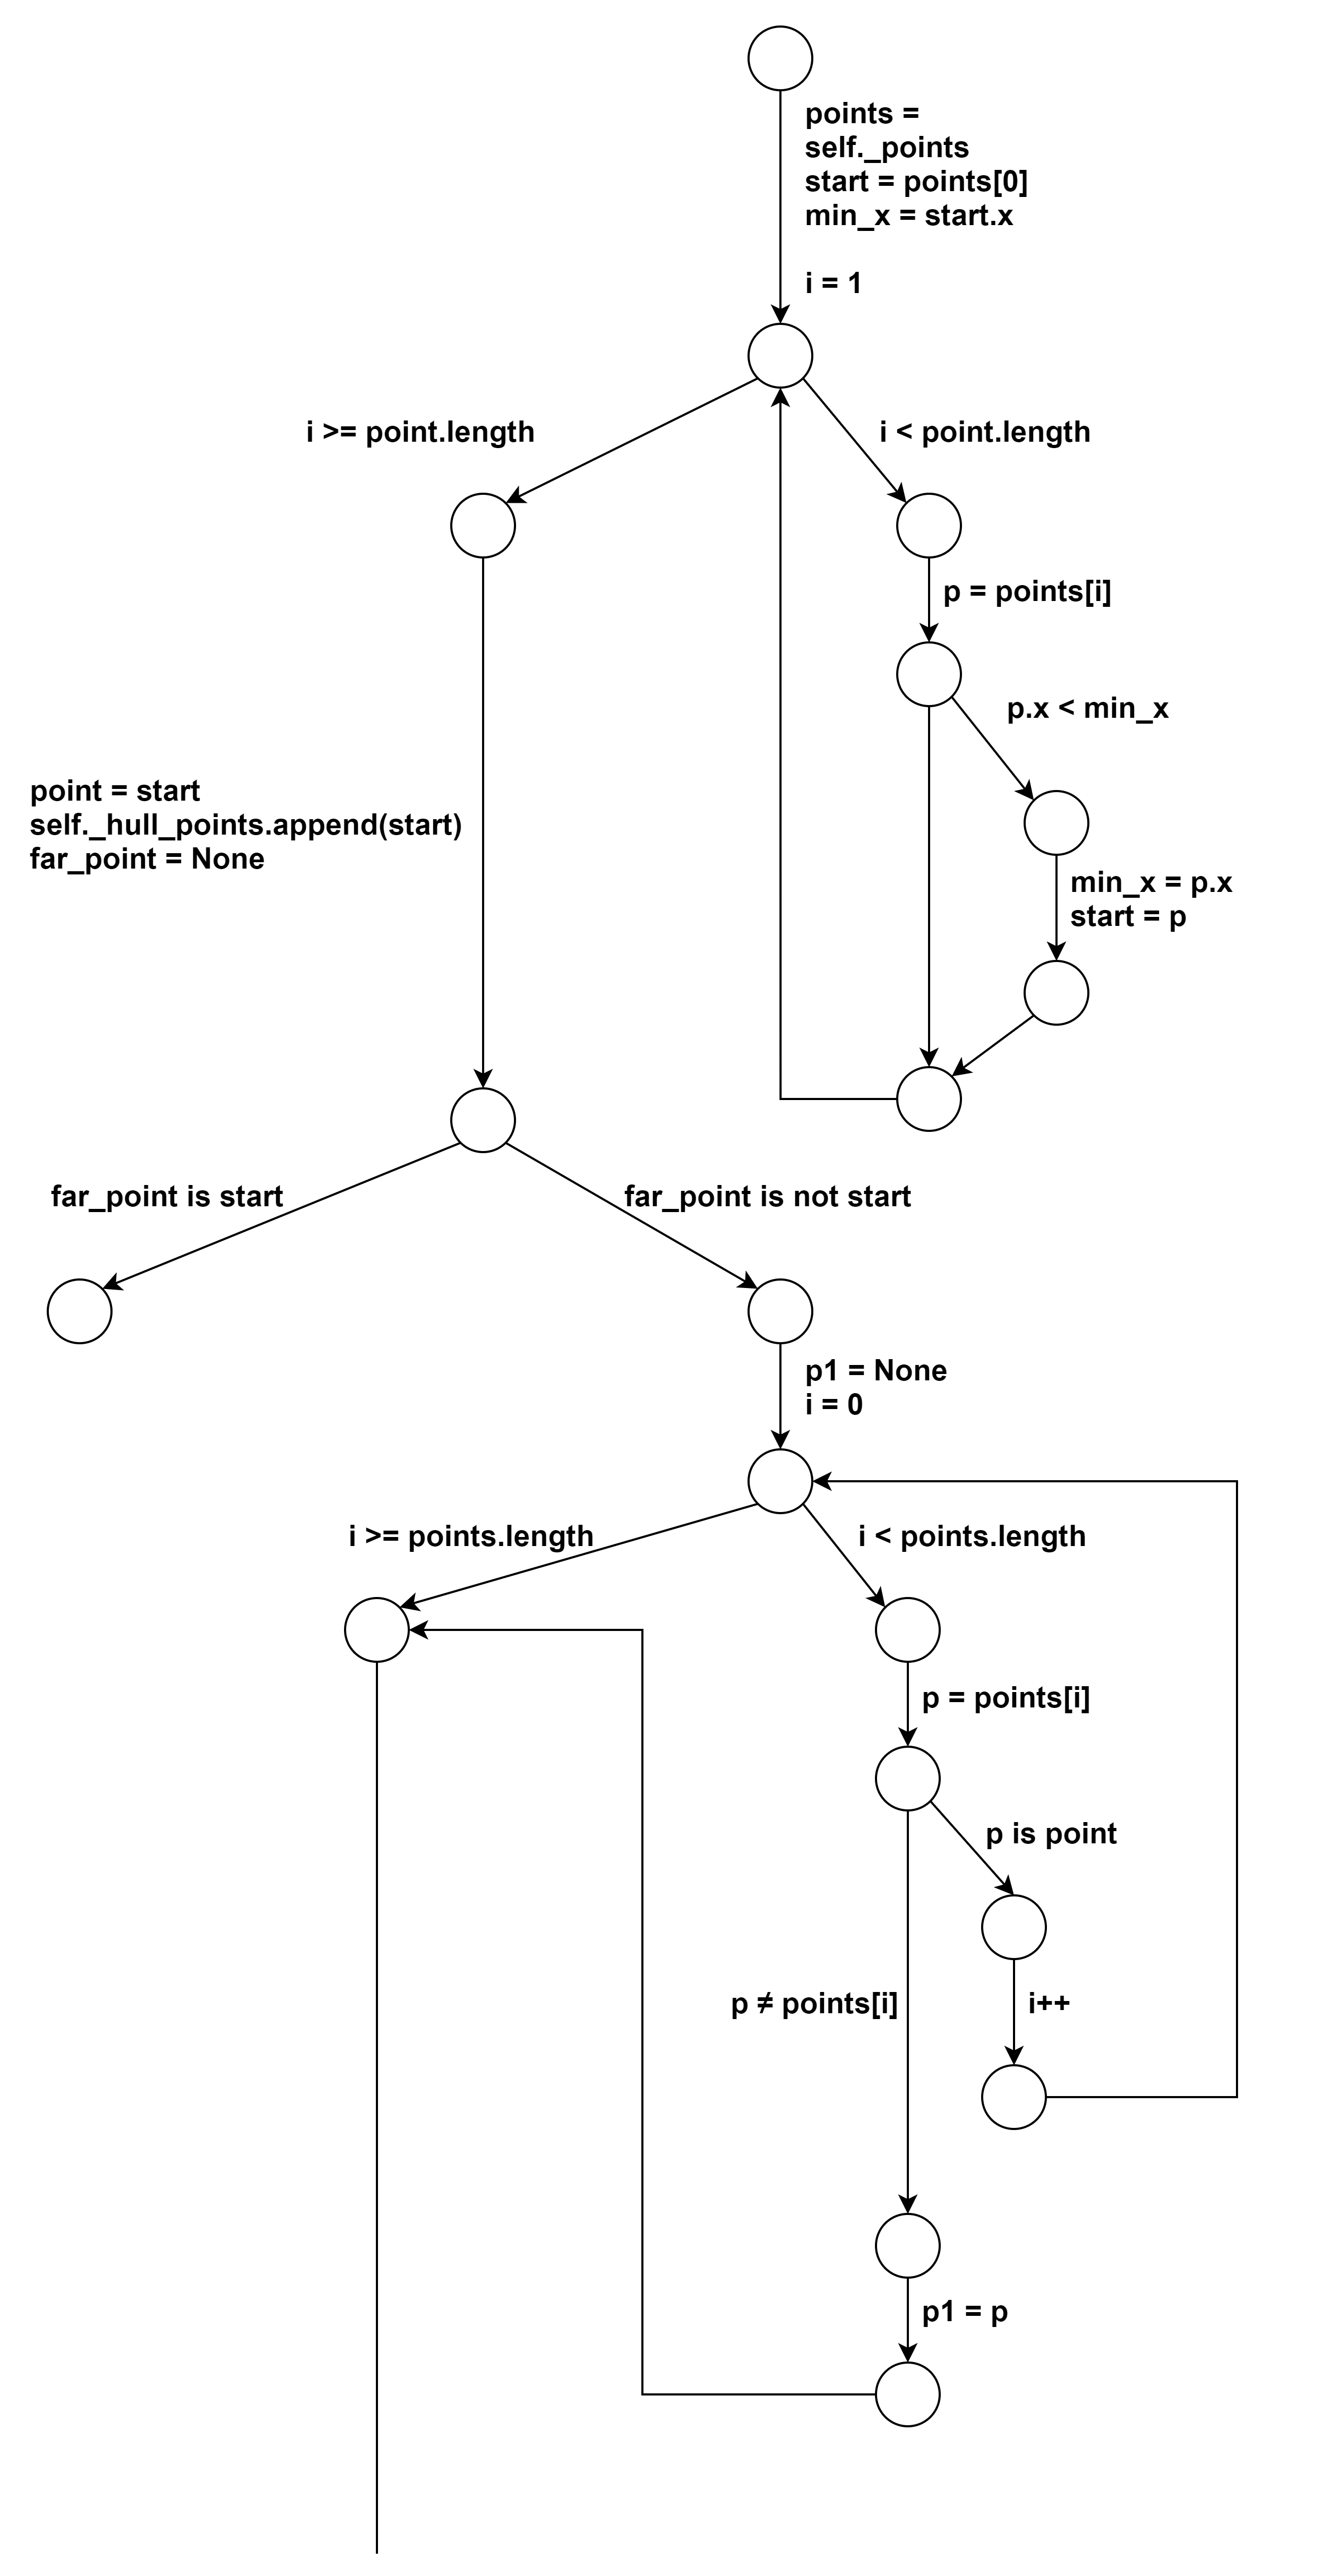
\includegraphics[width=0.7\textwidth]{Figures/Q2_1.png}
  \caption{Question 2. Control flow graph for convex hull(1) - continue}
\end{figure}

\begin{figure}[h!]
  \centering
  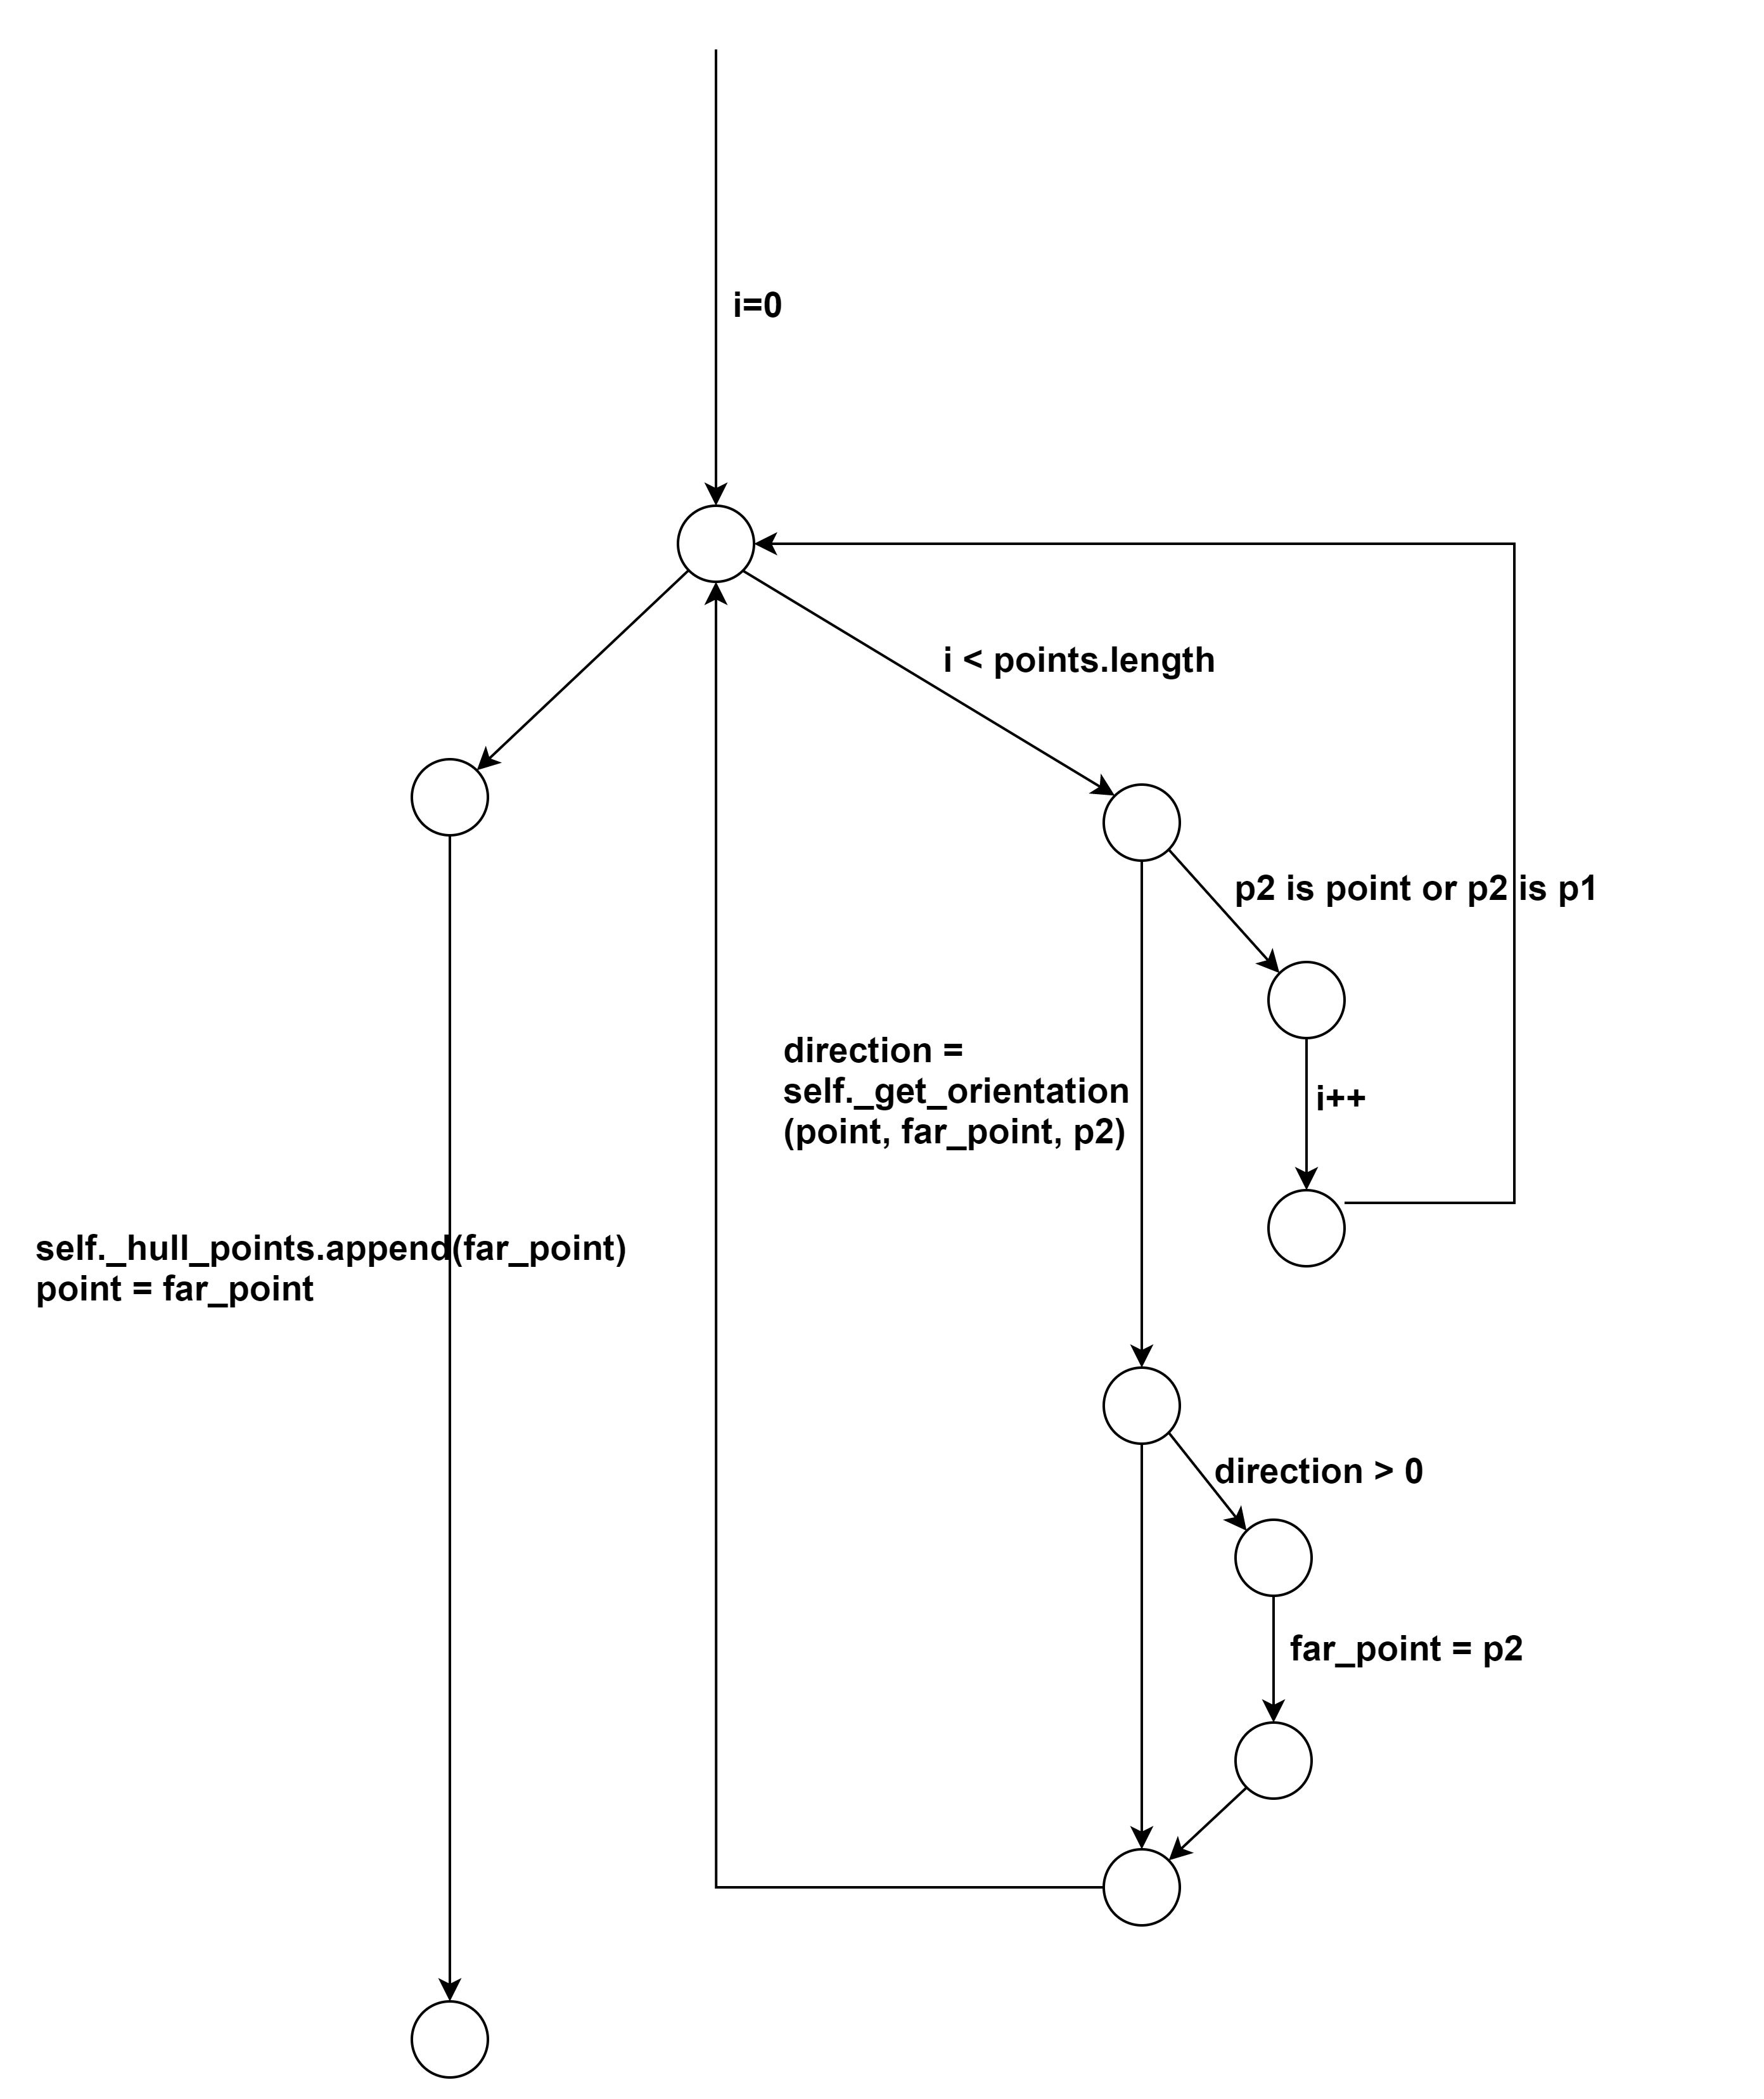
\includegraphics[width=0.7\textwidth]{Figures/Q2_2.png}
  \caption{Question 2. Control flow graph for convex hull(2)}
\end{figure}

\bigskip

\newpage
\clearpage
\begin{thebibliography}{9}
\bibitem{Bill} 
2020 Assignment 4, Design Specification (two-dots),\\
\texttt{Written by ``Bill Song''}

\bibitem{UML} 
UML diagram,\\
\texttt{https://app.diagrams.net/}

\bibitem{2048} 
2048,\\
\texttt{https://play2048.co/}

\bibitem{design} 
design strategy pattern,\\
\texttt{https://sourcemaking.com/design\_patterns/strategy}
\end{thebibliography}

\end {document}